\documentclass[11pt,a4paper]{article}
\usepackage[margin=2.3cm]{geometry}
\usepackage[T1]{fontenc}
\usepackage{lmodern}
\usepackage{amsmath,amssymb}
\usepackage{graphicx}
\usepackage{booktabs}
\usepackage[hidelinks]{hyperref}
\usepackage[numbers]{natbib}
\graphicspath{{../figures/}}

\title{Learning a Model and Controlling with It:\\
GP-MPC, DeePC and Koopman MPC on Three Simulated Plants}
\author{Arshia Goshtasbi\\Iran University of Science and Technology}
\date{November 2026}

\begin{document}
\maketitle

\begin{abstract}
This report describes a small benchmark of data-driven predictive controllers.
Three plants with a known structure but wrong parameters (a mass-spring-damper,
an inverted pendulum and a planar quadrotor with unknown drag and wind) are
controlled by five controllers under the same horizon, weights, input limits and
soft state constraints: MPC on the wrong prior model, MPC on the true model (an
oracle), MPC on the prior model plus a Gaussian-process residual (GP-MPC),
regularised data-enabled predictive control (DeePC) and linear MPC on a
Koopman (EDMD) lifted model. All learned components use the same 1500
noisy samples per seed. Over 10 seeds, the three learned controllers remove
most of the steady-state offset that the prior model leaves. GP-MPC has the
fewest constraint violations, the Koopman controller is the fastest by an
order of magnitude, and DeePC is the weakest on the quadrotor. Everything here is simulation; the claims are
limited to what the experiments measured.
\end{abstract}

\section{Problem setup}
Each plant is a continuous-time model $\dot x = f(x,u;\theta)$ simulated with
RK4 (10 sub-steps per sampling period $T_s = 0.05$\,s) under a zero-order-hold
input. The prior parameters $\theta_0$ differ from the true parameters
$\theta^\star$ (Table~\ref{tab:plants}). The state is measured with additive
Gaussian noise. Every controller solves, at each step, a finite-horizon problem
with horizon $N=20$,
\begin{equation}
\min \sum_{k=0}^{N-1} \|x_k-r_k\|_Q^2 + \|u_k-u^{\mathrm{ref}}\|_R^2 + \|x_N-r_N\|_{Q_f}^2
+ \rho_1 \mathbf{1}^\top s + \rho_2\|s\|^2,
\end{equation}
with hard input bounds and the state constraints $x^{\min}\le Cx_k\le x^{\max}$
softened by slacks $s\ge 0$ ($\rho_1=10^3$, $\rho_2=10^4$). The input reference
$u^{\mathrm{ref}}$ is the equilibrium input of the current set-point under the
prior model (under the true model for the oracle). Constraint violations are
measured afterwards on the true, noise-free state.

\begin{table}[h]
\centering
\caption{Plants and model mismatch.}
\label{tab:plants}
\small
\begin{tabular}{llp{6.2cm}}
\toprule
Plant & State / input & Mismatch (true vs prior) \\
\midrule
Mass-spring-damper & $(p,v)$ / $F$ & $k$: 2.0 vs 0.8, $c$: 0.4 vs 0.1, $m$: 1.0 vs 0.7 \\
Inverted pendulum & $(\theta,\omega)$ / $\tau$ & $m$: 1.0 vs 0.6; viscous and Coulomb friction unknown \\
Planar quadrotor & $(p_x,p_z,\phi,v_x,v_z,\omega)$ / $(T_1,T_2)$ & $m$: 1.0 vs 0.8; drag 0.4 and wind 0.6\,N unknown \\
\bottomrule
\end{tabular}
\end{table}

\paragraph{Data.} The pendulum and the quadrotor are open-loop unstable, so the
data are collected in closed loop: an LQR designed on the prior model tracks
random set-points (changed every 25 steps) while a Gaussian dither is added to
the input. Each dataset has 15 episodes of 100 steps (1500 samples). Seed $s$
draws the dataset; the closed-loop noise uses seed $500+s$.

\section{Controllers}
\paragraph{Nominal and oracle MPC.} Multiple-shooting NMPC on the RK4
discretisation (one sub-step) of the prior or the true model, solved with
IPOPT~\cite{wachter2006ipopt} through CasADi~\cite{andersson2019casadi}, warm
started with the shifted previous solution.

\paragraph{GP-MPC.} The mismatch enters through the accelerations, so one GP
per velocity state learns the one-step error
$\Delta v = v_{k+1} - F_0(x_k,u_k)_v$ from features $z=(x_k^{\mathrm{f}},u_k)$,
where $x^{\mathrm{f}}$ leaves out translation-invariant positions. The prediction
model is $x_{k+1} = F_0(x_k,u_k) + E\,\mu(z_k)$ with $E$ mapping $\Delta v$ to
the velocities and $\tfrac{T_s}{2}\Delta v$ to the positions. Each GP has a
squared-exponential ARD kernel with hyperparameters from the marginal
likelihood~\cite{rasmussen2006gpml}, trained on a random subset of 150 of the
1500 samples (a subset-of-data approximation). The constraints are tightened
by $\beta=2$ standard deviations, in the spirit of cautious
MPC~\cite{hewing2020cautious}: the GP variance is evaluated along the shifted
previous solution and summed over the horizon, ignoring the Jacobian of the
dynamics. \emph{This margin is a heuristic, not a certified bound.}

\paragraph{DeePC.} Following~\cite{coulson2019deepc}, the predictor is a
Hankel matrix of measured input--output data. With $w_k=(u_k,y_{k+1})$ and
$L = T_{\mathrm{ini}}+N$ ($T_{\mathrm{ini}}=3$), columns from all 15 episodes
form a mosaic Hankel matrix~\cite{vanwaarde2020lemma} (800 columns sampled at
random). The QP
\begin{equation}
\min_{g,\sigma}\ J(u,y) + \lambda_g\|g\|^2 + \lambda_\sigma\|\sigma\|^2
\quad\text{s.t.}\quad
\begin{bmatrix}U_p\\Y_p\\U_f\\Y_f\end{bmatrix} g =
\begin{bmatrix}u_{\mathrm{ini}}\\y_{\mathrm{ini}}+\sigma\\u\\y\end{bmatrix}
\end{equation}
is solved with OSQP~\cite{stellato2020osqp}. For a noise-free LTI system with
persistently exciting data, the fundamental lemma~\cite{willems2005note} makes
the Hankel predictor exact; a unit test checks this on the mass-spring-damper
(error below $10^{-5}$). For the nonlinear plants and for noisy data the
quadratic regularisation is a heuristic; guarantees for that setting need the
extra assumptions and terminal ingredients of~\cite{berberich2021datadriven},
which are not implemented here. The weight $\lambda_g$ was picked from
$\{0.01,0.1,1,10,100\}$ on a separate tuning seed by a fixed rule
(Fig.~\ref{fig:sweep}).

\paragraph{Koopman MPC.} EDMD~\cite{williams2015edmd} with inputs, as
in~\cite{korda2018linear}: $\psi(x) = (x, 1, \varphi_1(x),\dots,\varphi_{40}(x))$
with Gaussian radial basis functions on the standardised features, and
$\psi(x_{k+1}) \approx A\psi(x_k) + Bu_k$ fitted by ridge least squares. Since
$x$ is part of $\psi$, $x = C\psi$ with $C=[I\ 0]$, and the MPC is a condensed
QP solved with OSQP. The case without basis functions is the affine DMDc
model~\cite{proctor2016dmdc}, used as an ablation.

\section{Results}
\paragraph{Prediction.} Figure~\ref{fig:ident} and Table~\ref{tab:ident}
show the open-loop prediction error on held-out episodes. All learned models
improve on the prior model by one to two orders of magnitude. On the pendulum,
which is open-loop unstable, every model drifts after 20 steps; the Hankel
predictor drifts least. The radial basis functions improve on the affine DMDc
model only on the pendulum; on the mass-spring-damper DMDc is slightly better
and on the quadrotor the two are equal to three digits. The GP $2\sigma$ interval covered 94--96\,\% of
held-out one-step residuals.

\begin{figure}[h]
\centering
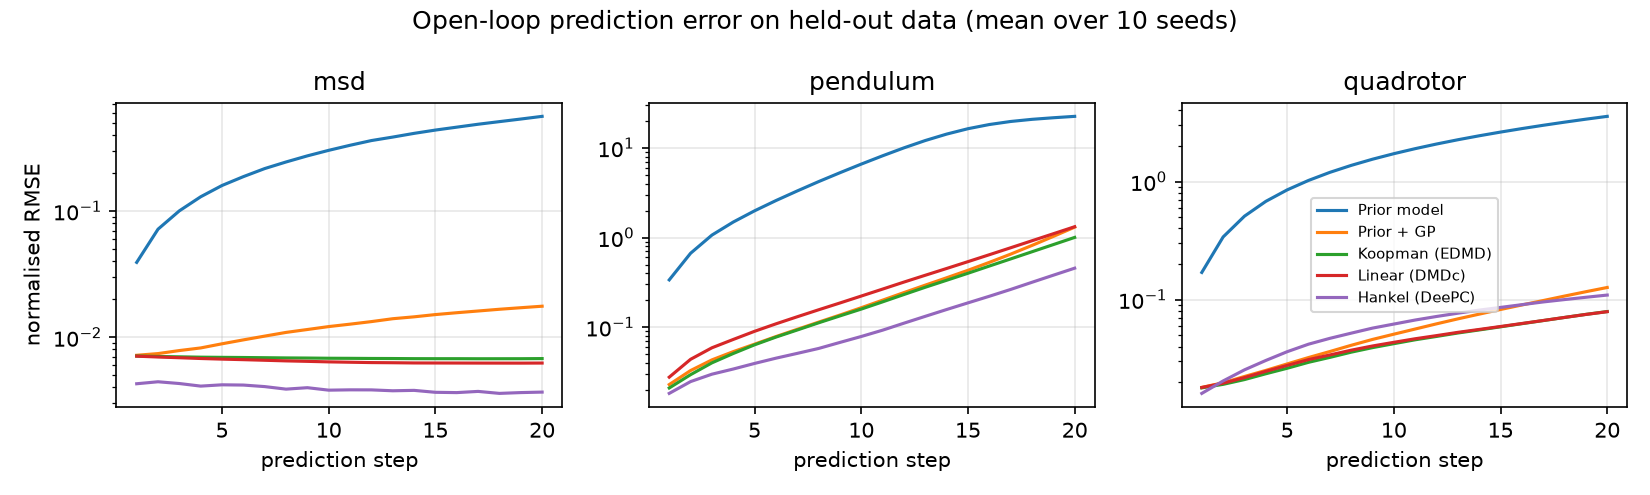
\includegraphics[width=\textwidth]{identification.png}
\caption{Open-loop prediction error versus horizon (held-out data, mean over 10 seeds).}
\label{fig:ident}
\end{figure}

\begin{table}[h]
\centering
\caption{Normalised RMSE at prediction step 20 and GP coverage.}
\label{tab:ident}
\small
\begin{tabular}{lccc}
\toprule
Model & msd & pendulum & quadrotor \\
\midrule
Prior model & 0.563 & 22.480 & 3.562 \\
Prior + GP & 0.018 & 1.306 & 0.127 \\
Koopman (EDMD) & 0.007 & 1.003 & 0.079 \\
Linear (DMDc) & 0.006 & 1.320 & 0.079 \\
Hankel (DeePC) & 0.004 & 0.455 & 0.109 \\
\midrule
GP $2\sigma$ coverage & 0.959 & 0.951 & 0.940 \\
\bottomrule

\end{tabular}
\end{table}

\paragraph{Closed loop.} Table~\ref{tab:cl} gives the metrics over 10 seeds:
tracking cost (mean of $\|x-r\|_Q^2$), steady-state error (position error
before the reference preview reaches the next set-point), the largest
violation (mean over seeds), the number of steps with a violation and the mean
solve time.

\begin{table}[h]
\centering
\caption{Closed-loop results, mean over 10 seeds (cost: mean $\pm$ std).}
\label{tab:cl}
\small
\begin{tabular}{lccccc}
\toprule
Controller & Cost & SS error & Max viol. & Steps viol. & Time [ms] \\
\midrule
\csname @@input\endcsname results_table.tex
\end{tabular}
\end{table}

The main observations, all read from Table~\ref{tab:cl}:
\begin{itemize}
\item The prior model leaves a steady-state offset (0.042, 0.011 and 0.104 on
the three plants). All three learned controllers reduce it: GP-MPC and Koopman
MPC to 0.001--0.003, close to the oracle, and DeePC less on the quadrotor
(0.041).
\item GP-MPC has the cost closest to the oracle on the quadrotor and the
fewest violation steps on every plant (on the pendulum tied at zero with
nominal MPC and DeePC); it is the only controller that tightens the
constraints. It is also the slowest controller
on the quadrotor (49.5\,ms mean, close to the 50\,ms sampling time).
\item Koopman MPC is the fastest (below 1\,ms) and has the lowest cost on the
mass-spring-damper and the pendulum, but the largest violations on the
pendulum and the quadrotor (Fig.~\ref{fig:cl}: a sharp roll transient at the
start).
\item DeePC works with no model at all, but on the quadrotor it has the highest
cost and the largest spread across seeds, and on the mass-spring-damper its
worst-case solve time (234\,ms) exceeds the sampling time.
\item The oracle violates the soft constraints slightly on every plant, because
of measurement noise and because it has no margin.
\end{itemize}

\begin{figure}[h]
\centering
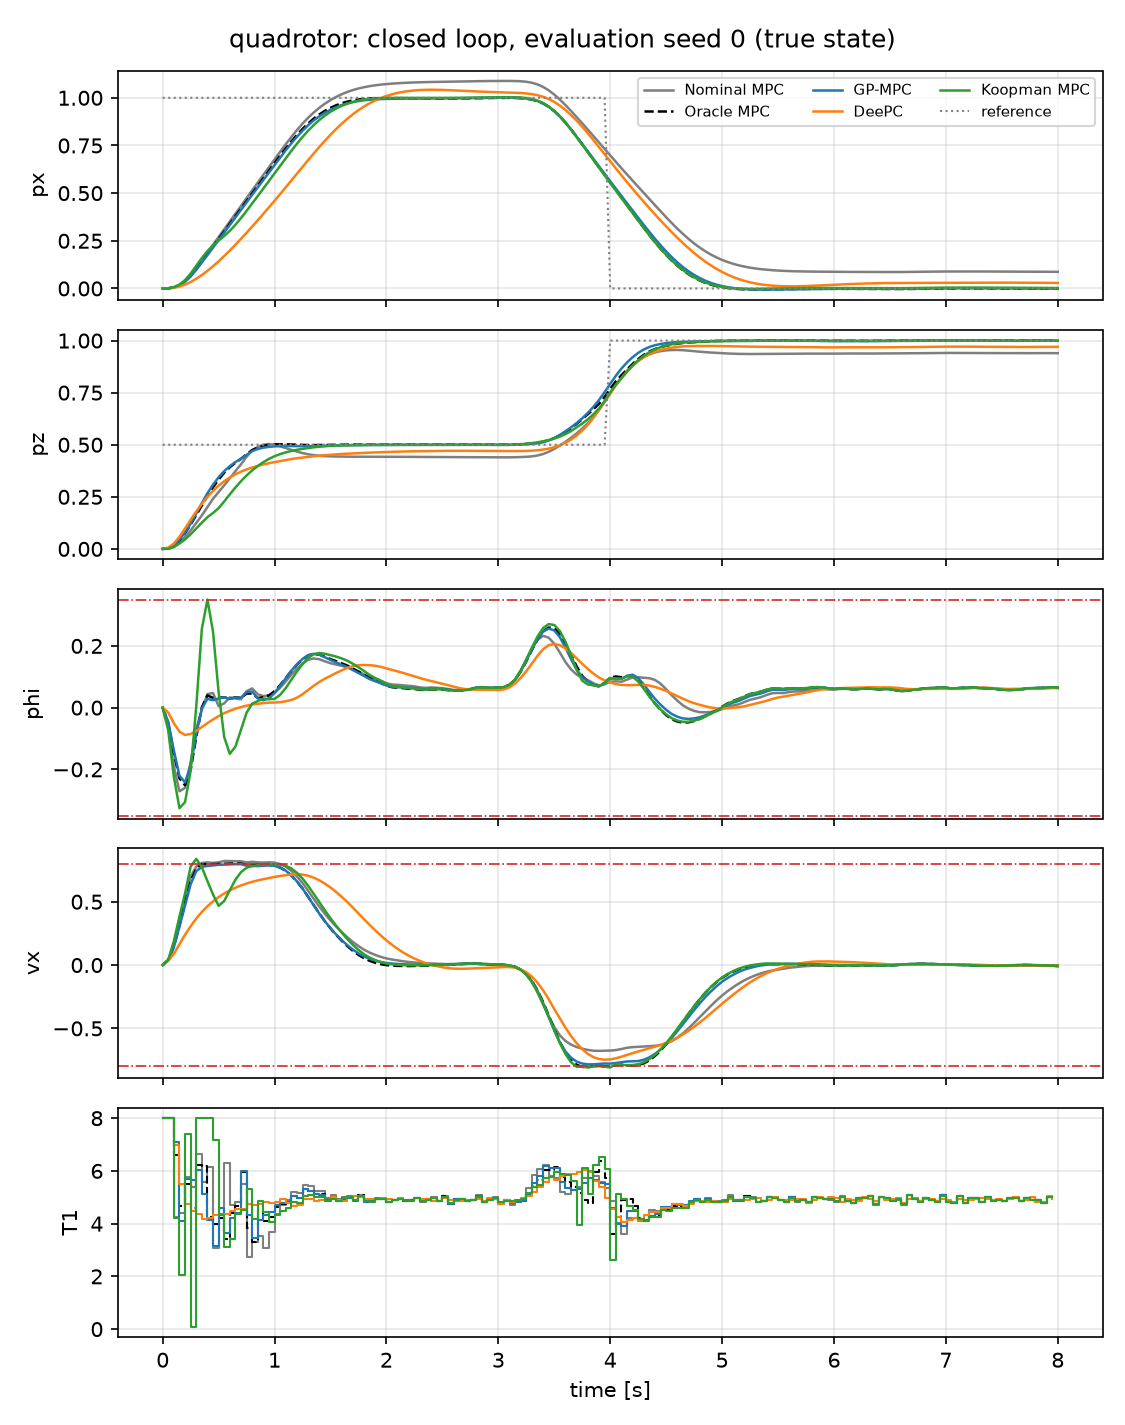
\includegraphics[width=0.75\textwidth]{closed_loop_quadrotor.png}
\caption{Quadrotor closed loop, evaluation seed 0. Dash-dot lines are the
state constraints.}
\label{fig:cl}
\end{figure}

\begin{figure}[h]
\centering
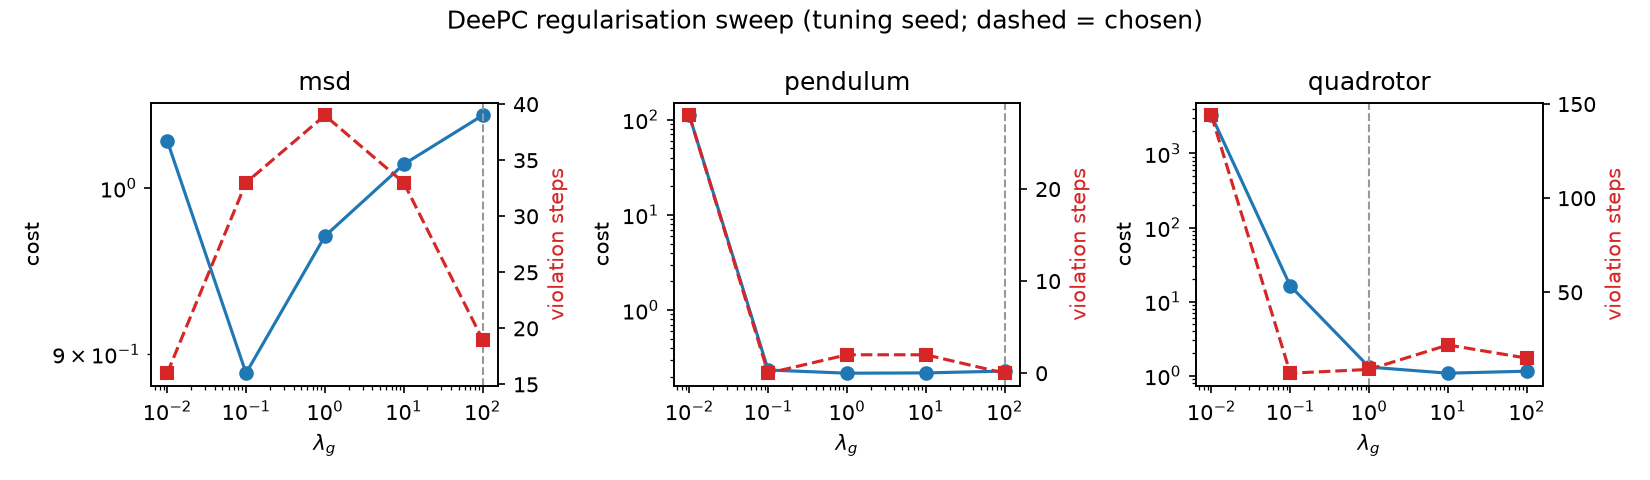
\includegraphics[width=\textwidth]{deepc_sweep.png}
\caption{DeePC regularisation sweep on the tuning seed (dashed: chosen weight).}
\label{fig:sweep}
\end{figure}

\section{Limitations}
Everything is simulated, with one mismatch scenario per plant and a fixed data
budget. The GP uses a subset of the data and its tightening ignores how
uncertainty propagates through the dynamics. DeePC and Koopman MPC carry no
closed-loop guarantee here. The tracking cost is dominated by the transients
after set-point changes, which all controllers share, so differences in cost
are small; the steady-state error and the violations separate the methods
more clearly.

\bibliographystyle{plainnat}
\bibliography{refs}
\end{document}
